\section{Monte Carlo Simulation}
 The Hall-A Single Arm Monte Carlo simulation tool (SAMC) was designed to simulate the transportation of particles from the target plane to the focal plane. SAMC was originally developed in FORTRAN~\cite{A_Duer} and then converted into C++~\cite{hyao_thesis}. The beam position, the spectrometer settings, and the information of the target system can be specified in the code to match the experimental settings. A simulated event has its specified values of the incoming energy, the scattered momentum and the scattering angle, which are defined in the target coordinate system and called the target plane quantities. These quantities are randomly generated with uniform distributions, and with these quantities as inputs, each focal plane quantity is calculated by a set of forward transportation functions which are generated by the SNAKE model~\cite{snack_lerose}. After the focal plane quantities are smeared with the resolution of VDCs, another set of backward transportation functions are used to reconstruct the target plane quantities. During these two processes, events inside and outside the HRS acceptance can be individually identified. Before comparing with the experimental data, the distributions of the target plane quantities are weighted by the radiated cross section values of these simulated events which can be calculated with cross section models embedded in the code. In this analysis, a new cross section model and a special treatment of the no-uniform cryogenic targets have been added in SAMC.

 There were 20 million events generated for each target in each kinematic setting. Fig.~\ref{samc_tg_c12} and Fig.~\ref{samc_tg_he3} compare the distributions of reconstructed target plane quantities between simulated data and experimental data for $\mathrm{^{12}C}$ and $\mathrm{^{3}He}$. The histograms for simulation data were weighted by the cross sections calculated by XEMC (see next section and Appendix B). The distribution of the same quantity from these two data sets agree nicely with each other. The distribution of $z_{react}$ for the cryogenic target was simulated with the relative density distribution function extracted with the method discussed in Appendix D.
\begin{figure}[!ht]
  \begin{center}
    \subfloat[Target plane quantities on HRS-L]{
      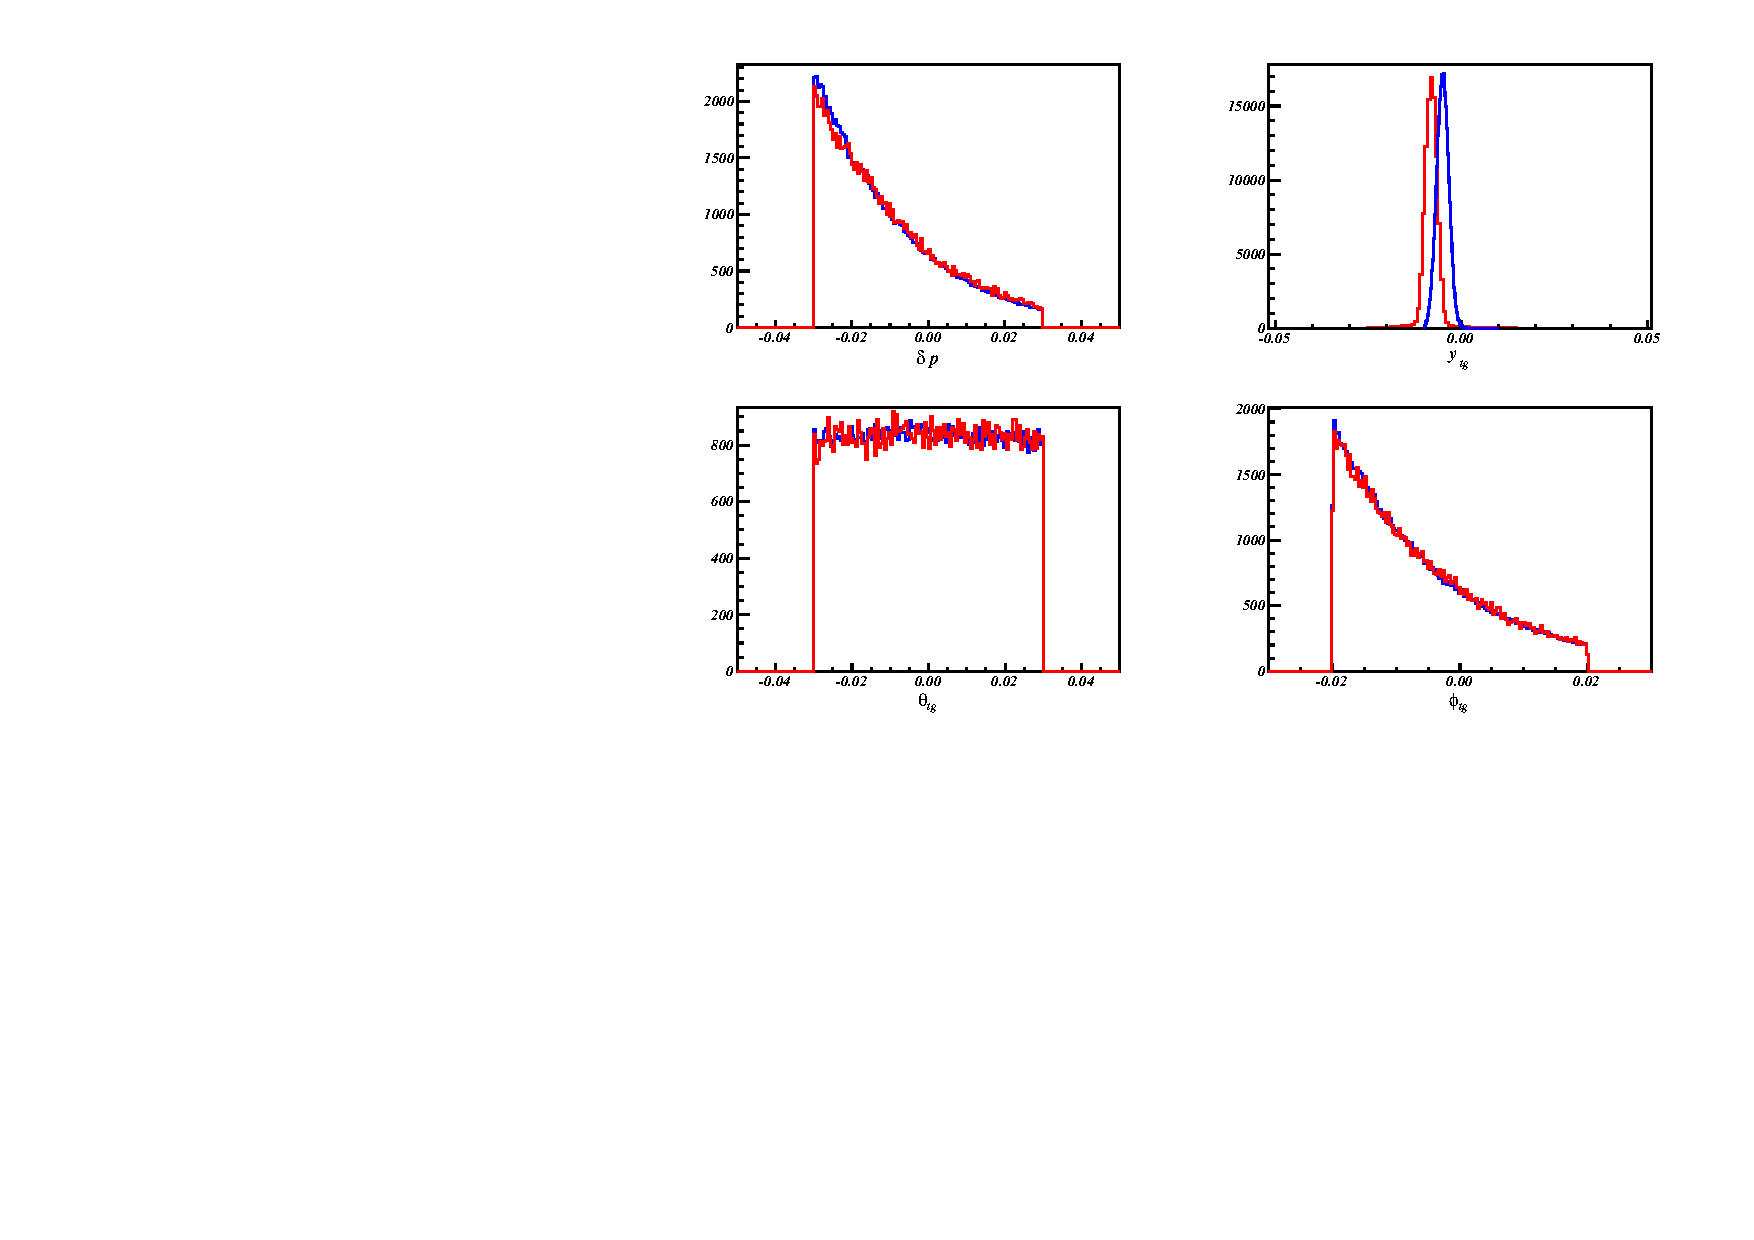
\includegraphics[type=pdf, ext=.pdf,read=.pdf,width=0.92\textwidth]{./figures/samc/C12_L_Kin51_TG}
    }
    \\
    \subfloat[Target plane quantities on HRS-R]{
      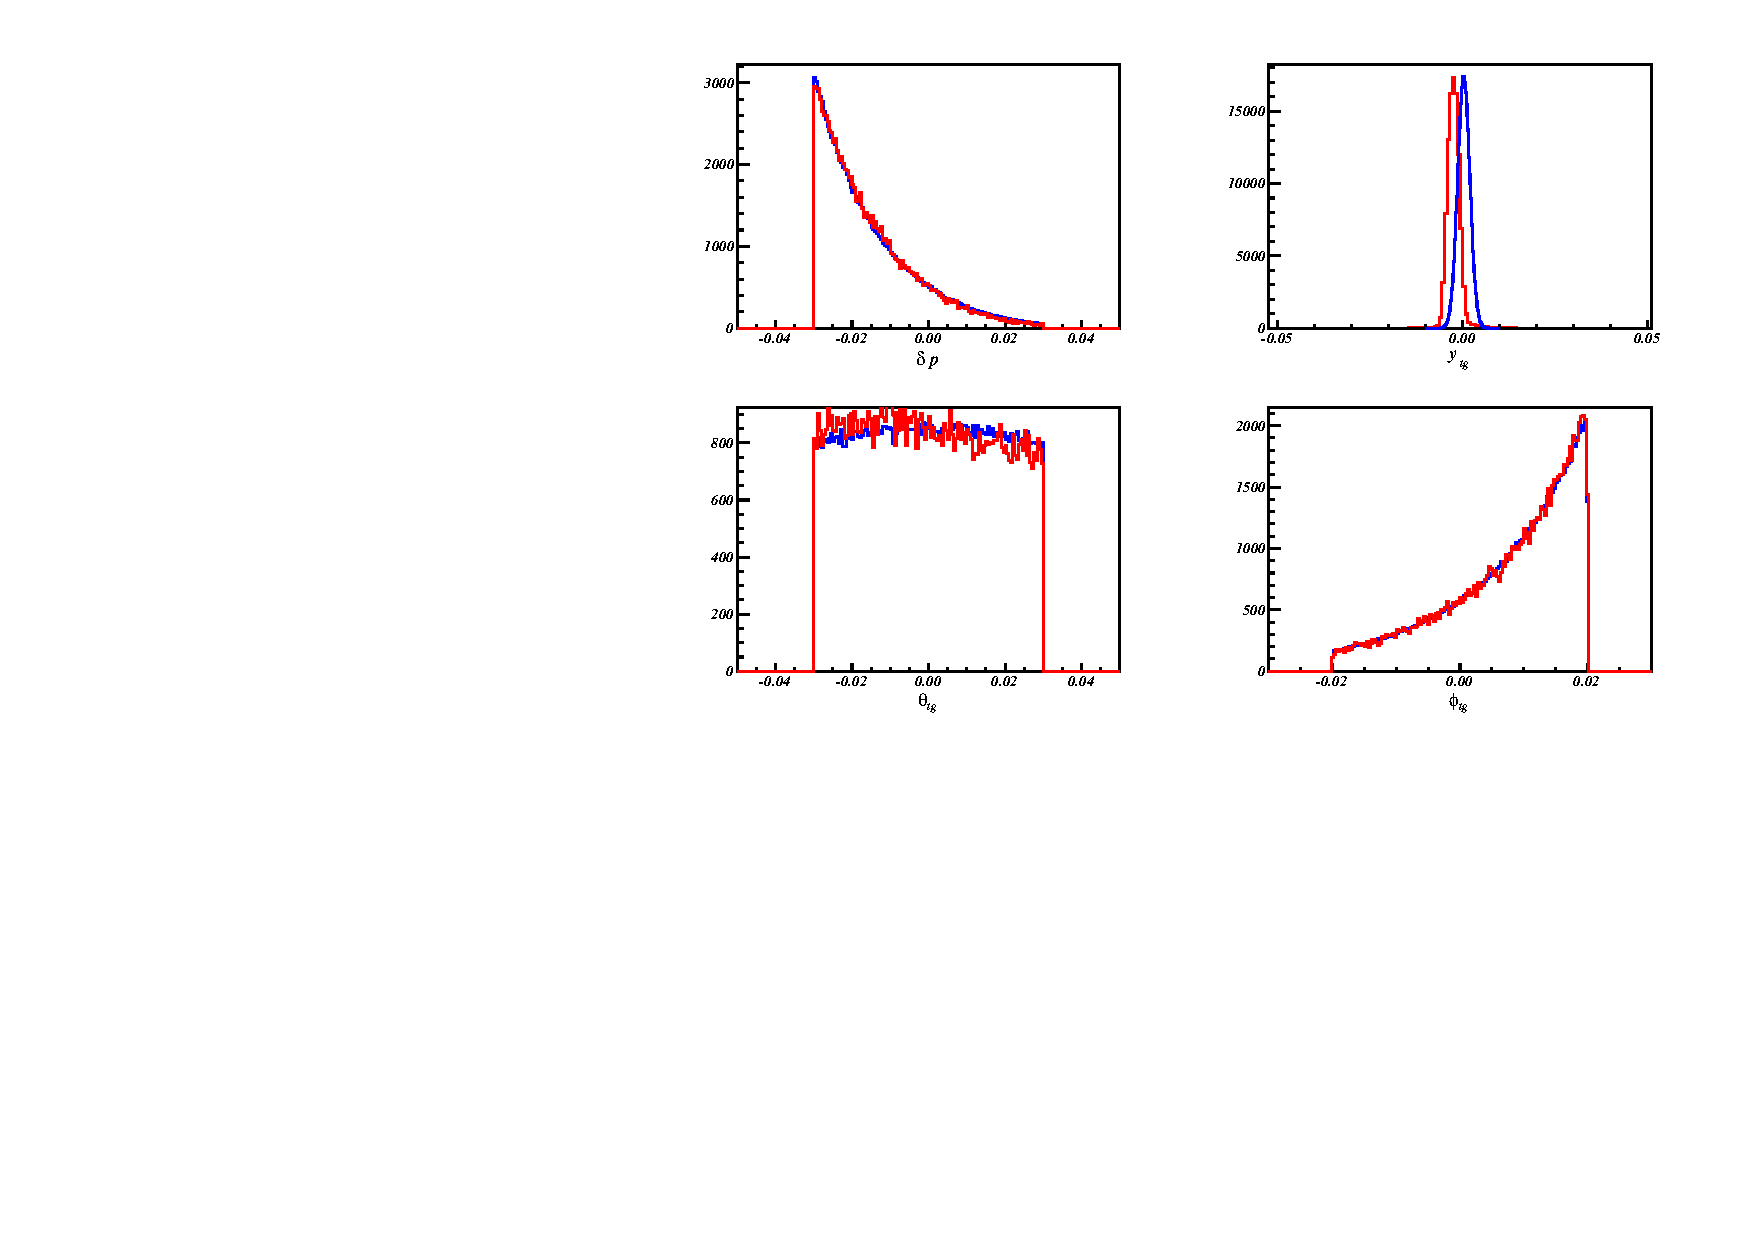
\includegraphics[type=pdf, ext=.pdf,read=.pdf,width=0.92\textwidth]{./figures/samc/C12_R_Kin32_TG}
    }
    \caption[Simulation of $\mathrm{^{12}C}$ target plane quantities]{\footnotesize{Simulation of $\mathrm{^{12}C}$ target plane quantities, where red lines are simulation data from SAMC and blue lines are from the E08-014 data. The offset of $y_{tg}$ between two data is a known issue of SAMC but the offset was too small to affect the acceptance.}}
    \label{samc_tg_c12}
  \end{center}
\end{figure}
\begin{figure}[!ht]
  \begin{center}
    \subfloat[Target plane quantities on HRS-L]{
      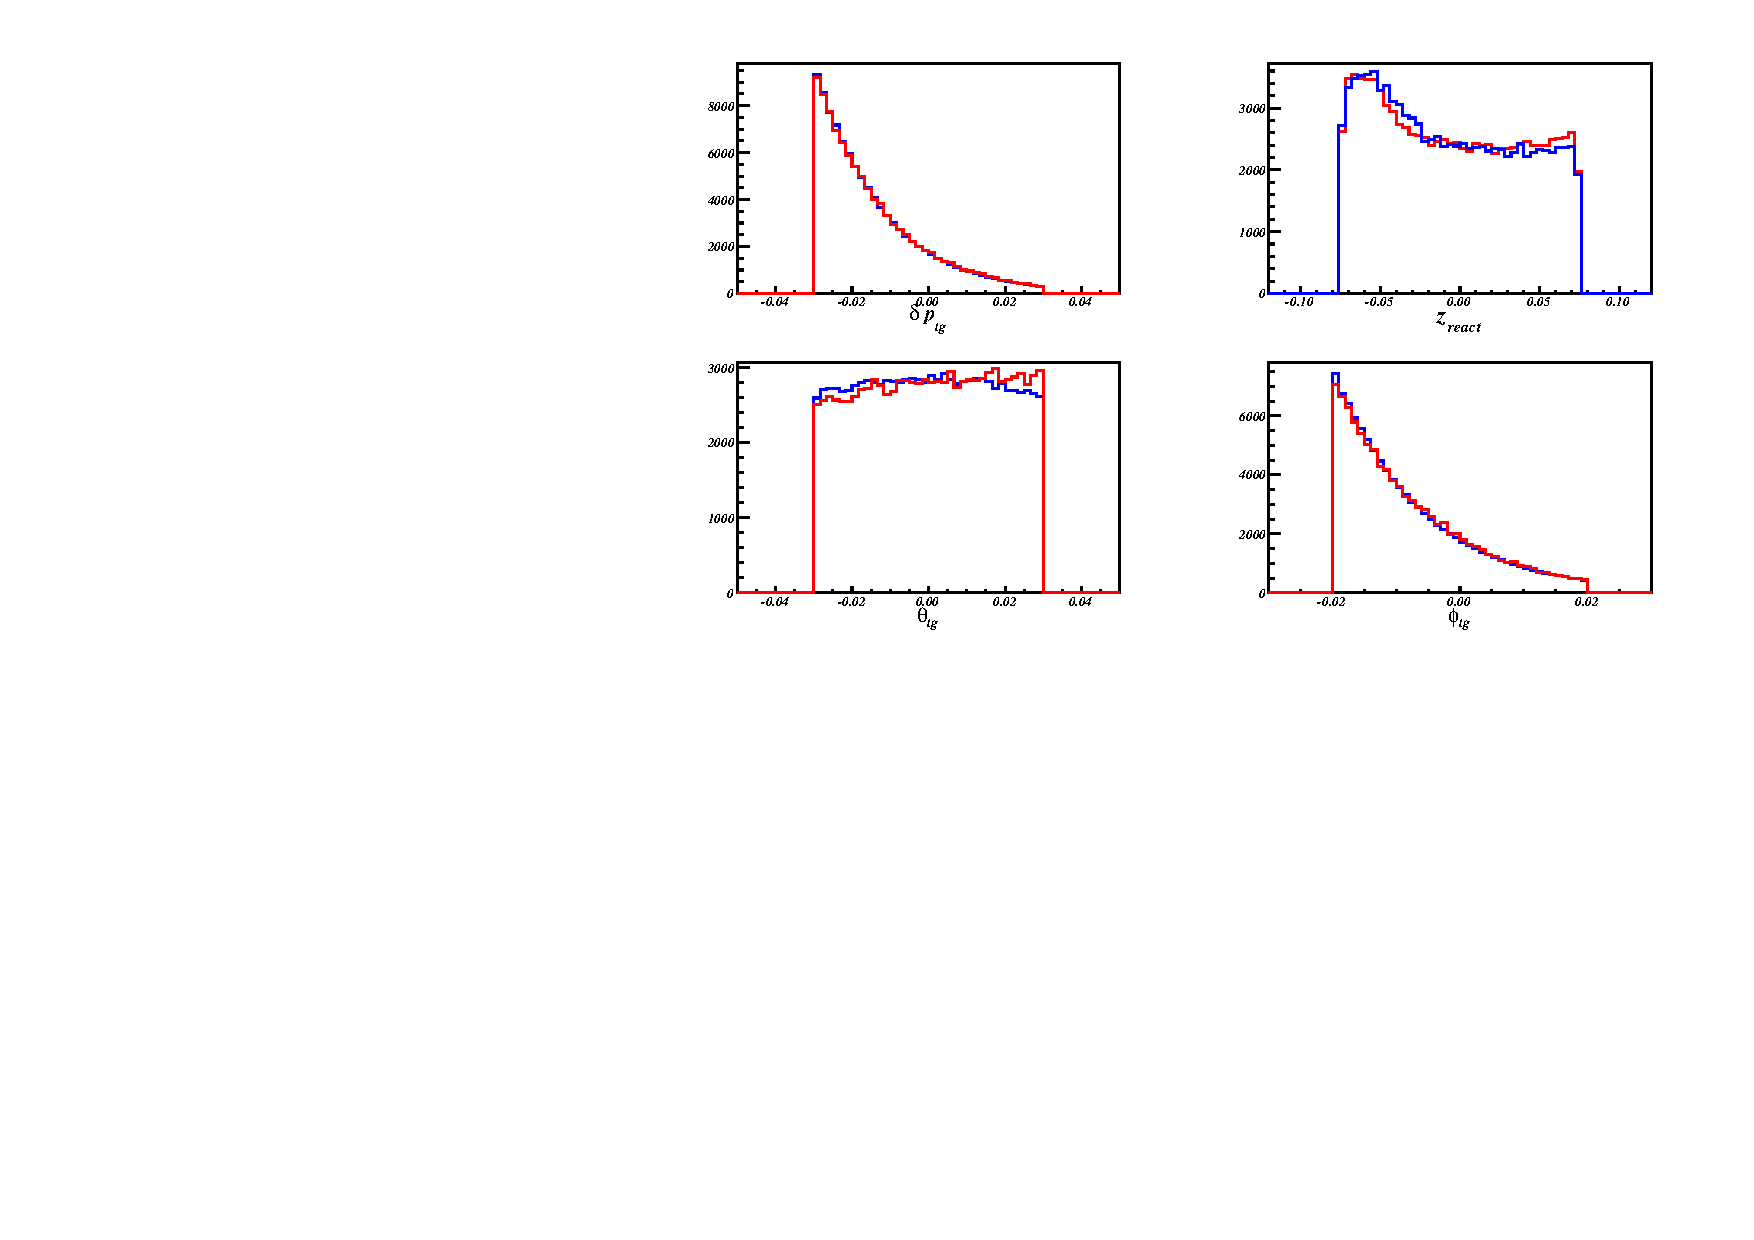
\includegraphics[type=pdf, ext=.pdf,read=.pdf,width=0.92\textwidth]{./figures/samc/He3_L_Kin31_TG}
    }
    \\
    \subfloat[Target plane quantities on HRS-R]{
      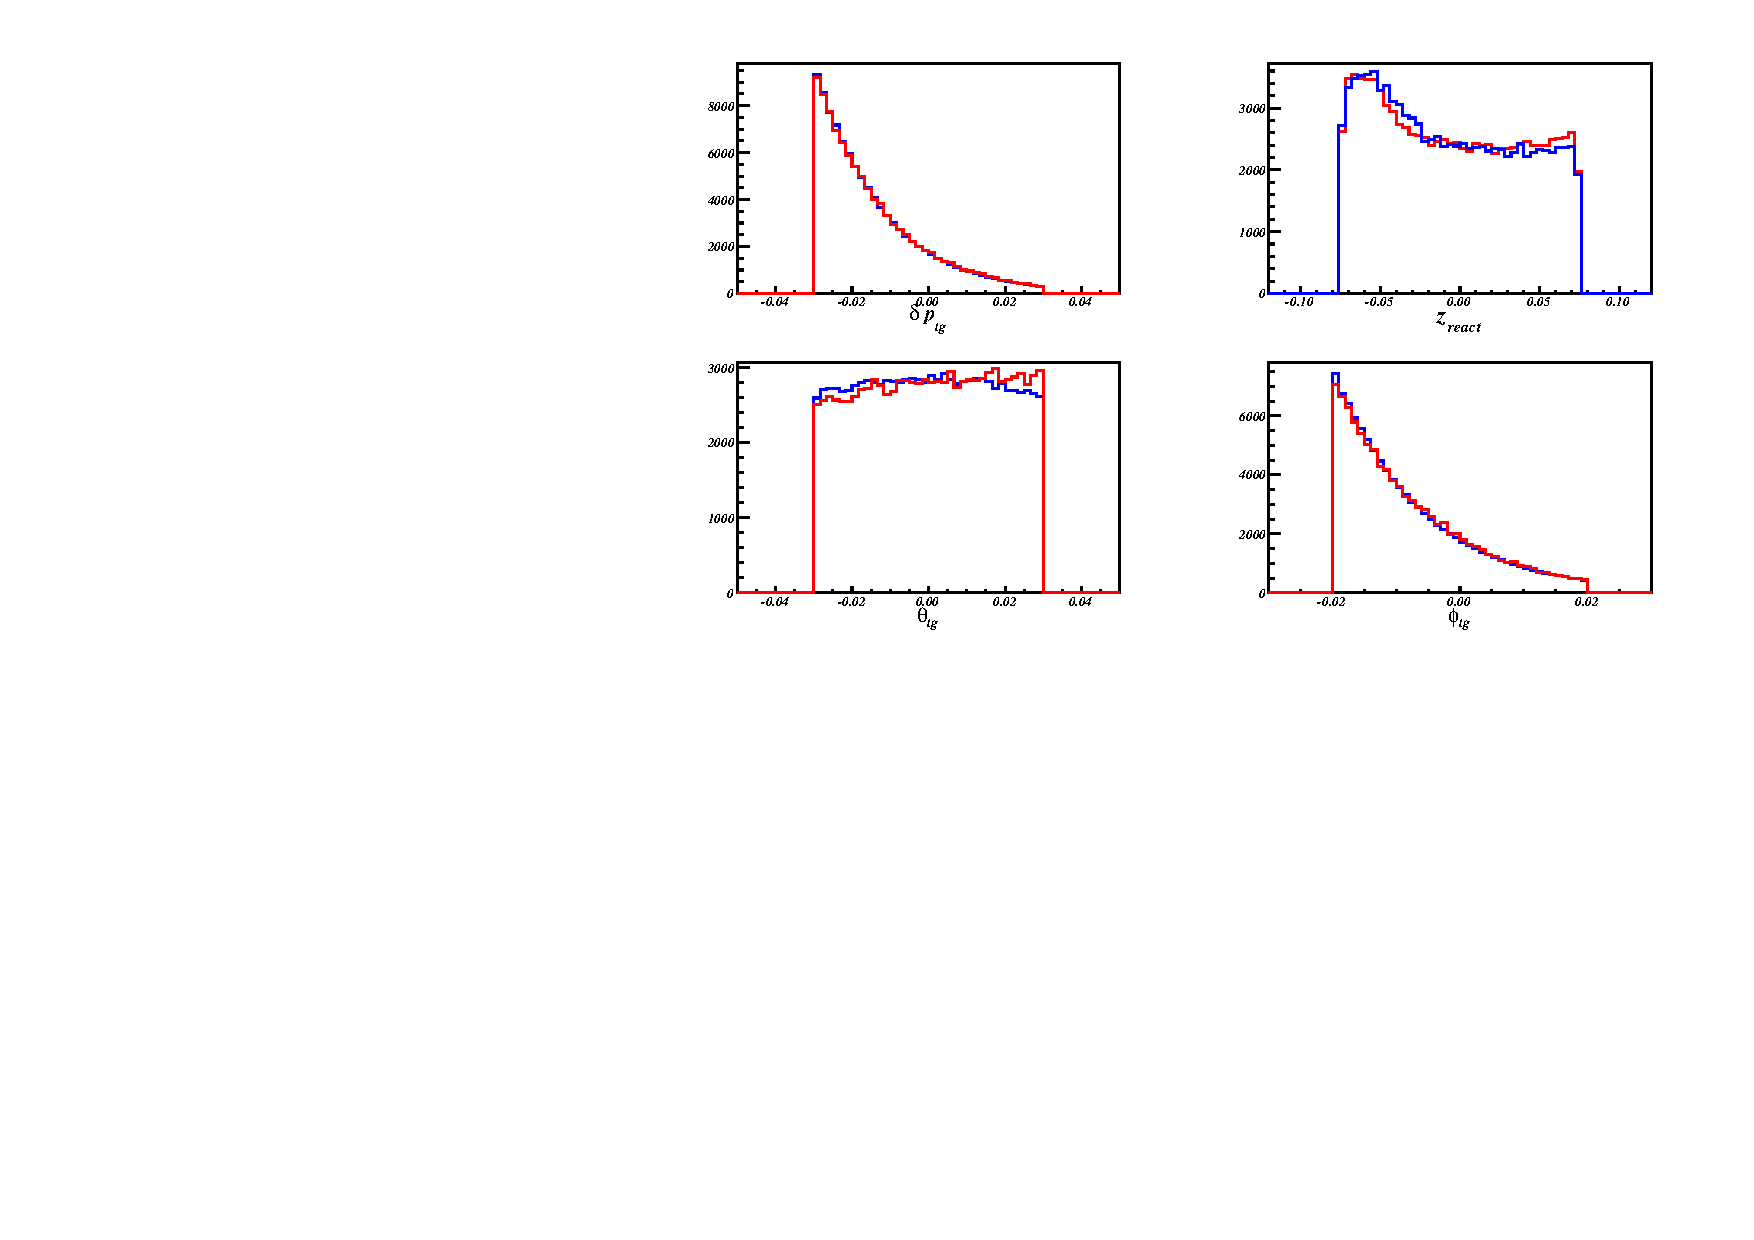
\includegraphics[type=pdf, ext=.pdf,read=.pdf,width=0.92\textwidth]{./figures/samc/He3_L_Kin31_TG}
    }
    \caption[Simulation of $\mathrm{^{3}He}$ target plane quantities]{\footnotesize{Simulation of $^{3}$He target plane quantities, where red lines are simulated data from SAMC and blue lines are the experimental data. Instead of $y_{tg}$, the $z_{react}$ distribution is given to compare the real density distribution which was simulated with the function fitted from data (Appendix D).}}
    \label{samc_tg_he3}
  \end{center}
\end{figure}

\section{Cross Section Model}
 The inclusive electron scattering cross sections model used in this data analysis is XEMC, a C++ package to compute Born cross sections and radiated cross sections. A brief discussion of the cross section models and radiative correction is given in Appendix B. 
\begin{figure}[!ht]
  \begin{center}
    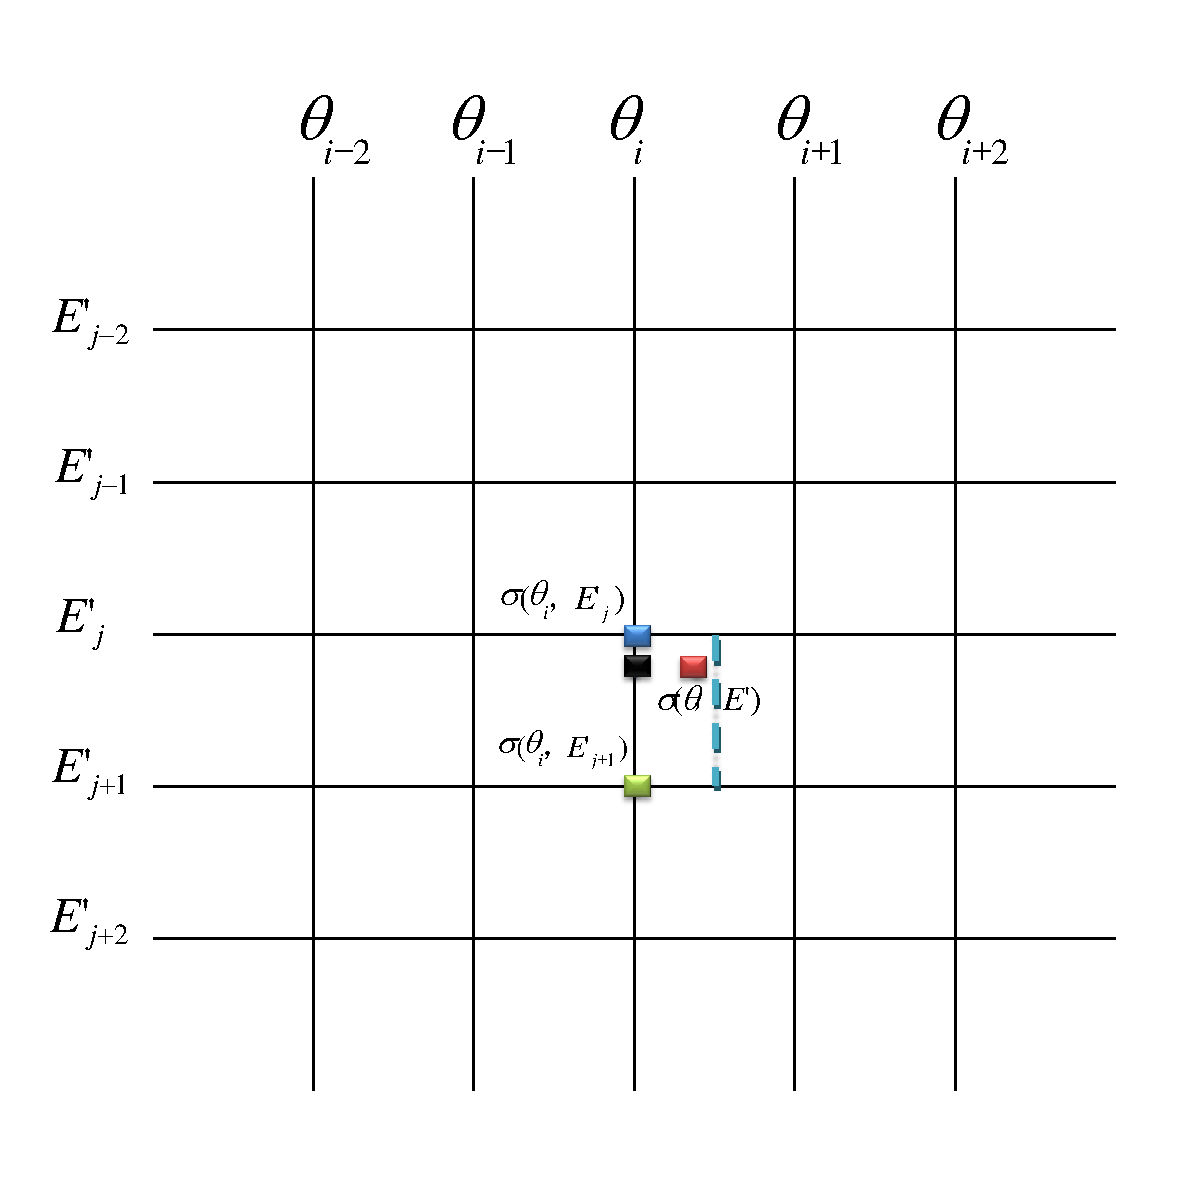
\includegraphics[type=pdf, ext=.pdf,read=.pdf,width=0.60\textwidth]{./figures/xemc/LookUp_Table}
    \caption[A sketch of cross section lookup tables]{\footnotesize{A sketch of cross section lookup tables. $\sigma(\theta,E') \equiv \sigma(\theta_{i},E')$ when $\theta_{i}\leq \theta < (\theta_{i}+\theta_{i+1})/2$, and $\sigma(\theta,E') \equiv \sigma(\theta_{i+1},E')$ when $(\theta_{i}+\theta_{i+1})/2\leq \theta <\theta_{i+1}$, e.g. from the red point to the black point in this plot. For $E'_{j}<E'<E'_{j+1}$, the cross section is calculated with the linear relationship given in Eq.~\eqref{xs_lookup_ep}.}}
    \label{xs_table}
  \end{center}
\end{figure}

 Calculating radiated cross sections with XEMC usually takes very long time. To generate millions of simulated events, cross section look-up tables were generated for each target in each kinematic setting. When generating each table, the range of the scattering angle, $\Delta\theta$, and the scattered energy, $\Delta E'$, were slightly wider than the actual HRS acceptance. $\Delta\theta$ was divided into 200 bins and $\Delta E'$ was also split into bins of 5 MeV. As shown in Fig.~\ref{xs_table}, the kinematic space for each setting was given as a 2-dimensional lattice where the born cross section and the radiated cross section for each grid, ($\theta_{i}$, $E'_{j}$), were simultaneously calculated. Since the bin sizes are very fine, for fixed momentum, the cross sections at different angles are considered to be equal within one $\theta$ bin, while for a fixed angle, the cross sections are assumed to be proportional to the momentum values inside one $E'$ bin. As illustrated in Fig.~\ref{xs_table}, for a given event, ($\theta,E'$), the value of $\theta$ is replaced by the closest angle bin, e.g. $\theta_{i}$, and when two momentum bins are specified, e.g. $E'_{j}<E'<E'_{j+1}$, the cross section value for this event can be calculated with the linear relationship:
\begin{equation}
  \sigma(E',\theta) = \sigma(E'_{j},\theta^{i}) - \frac{E'-E'_{j}}{E'_{j+1}-E'_{j}}\left(\sigma(E'_{j},\theta^{i})-\sigma(E'_{j+1},\theta^{i})\right).
  \label{xs_lookup_ep}
\end{equation}
For the same event, the difference between the cross section obtained from the look-up table and the cross section directly calculated from XEMC is less than 0.1\%. This method can dramatically reduce the computation time when generating simulation events. Tables were re-generated each time when the model was changed or the experimental details were updated, e.g. the target thickness.
